% Auto-generated by make_vlm_figures.py. Do not edit by hand.
% Copy the environments you need into the manuscript, or
% \input this file where the figures should appear.
%
% Figures are numbered in the order they are intended to appear.
% LaTeX renumbers automatically, so cross-reference with the
% \label keys below rather than with the file numbers.

% ---- figure0: pipeline ----
\begin{figure}[!htbp]
\centering
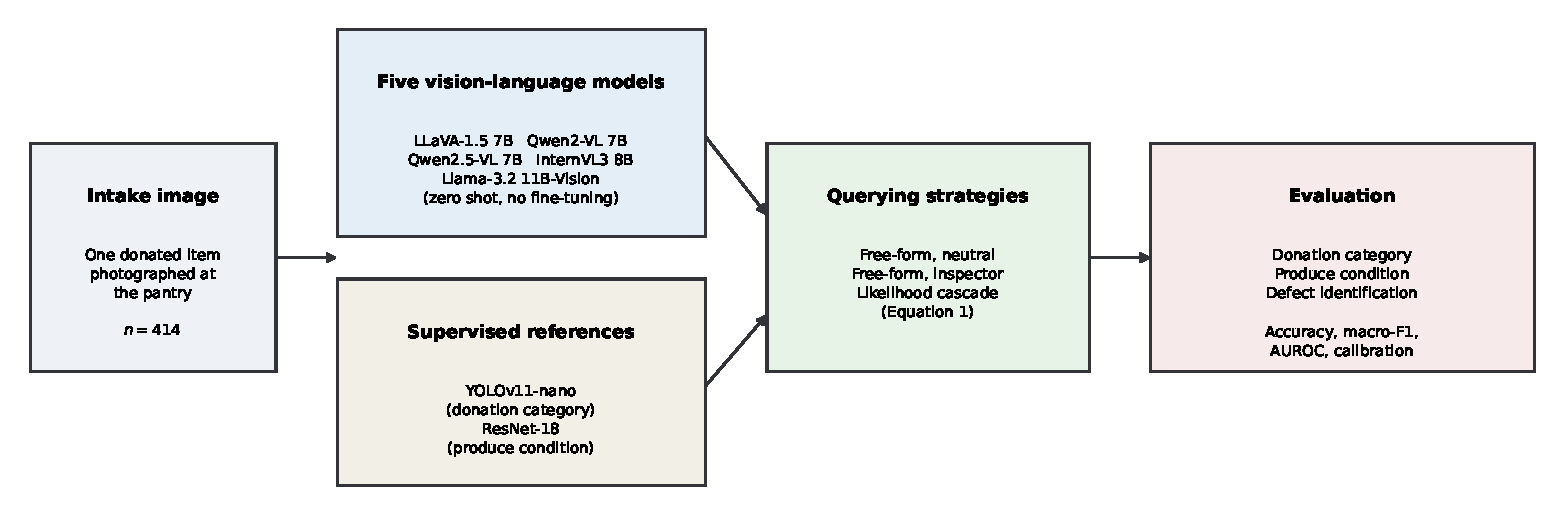
\includegraphics[width=\textwidth]{figures/figure0.pdf}
\caption{Evaluation framework. A single intake image of one donated item is presented to five open-weight vision--language models under three querying strategies (neutral free-form, rejection-oriented inspector, and the binary likelihood cascade of Eq.~\ref{eq:cascade}). Supervised YOLOv11 and ResNet-18 models trained on the same images provide references. All configurations are evaluated on donation category assignment, produce condition assessment, and defect identification.}
\label{fig:pipeline}
\end{figure}

% ---- figure1: donation_category ----
\begin{figure}[!htbp]
\centering
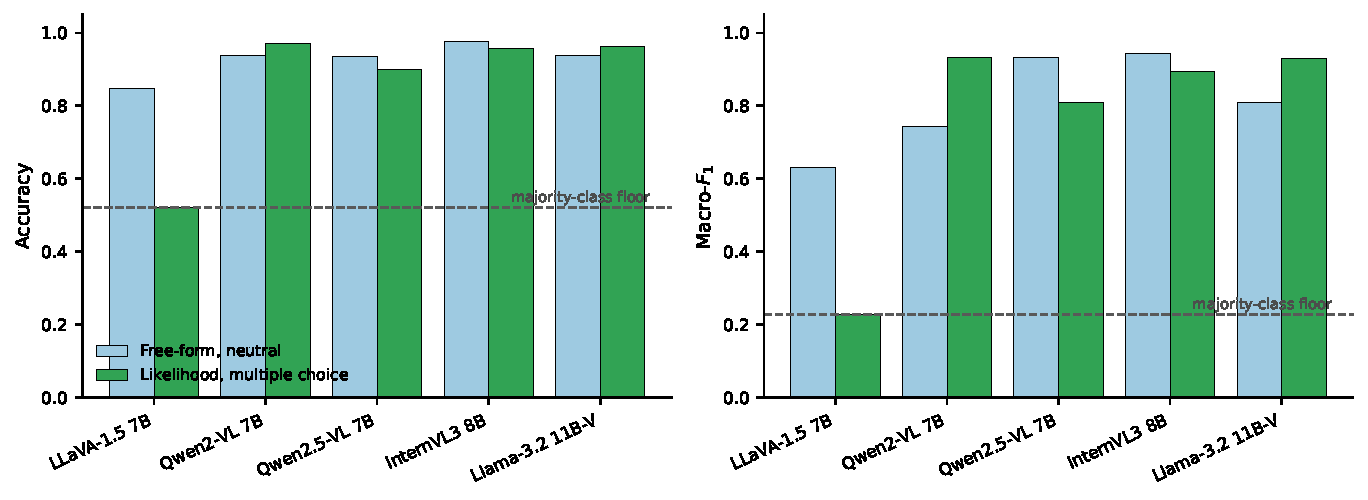
\includegraphics[width=\textwidth]{figures/figure1.pdf}
\caption{Donation category identification across five vision--language models and two querying strategies ($n = 414$). Left: accuracy. Right: macro-$F_1$. Dashed lines mark the majority-class floor. The two panels diverge because the bakery class has only 22 examples, so a model can reach high accuracy while recovering that class poorly.}
\label{fig:donation}
\end{figure}

% ---- figure2: condition_grid ----
\begin{figure}[!htbp]
\centering
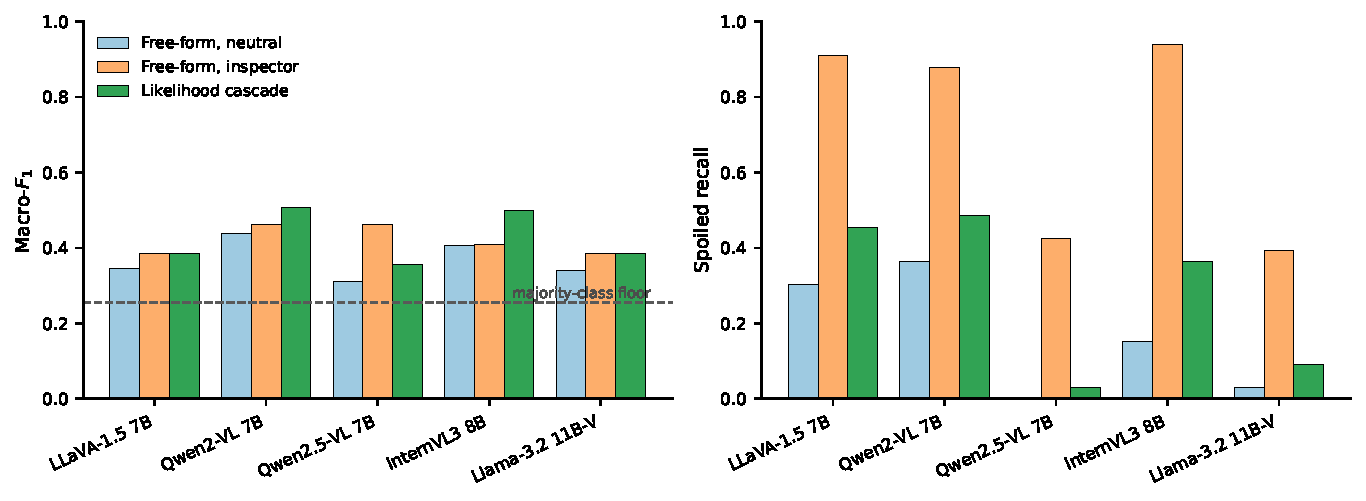
\includegraphics[width=\textwidth]{figures/figure2.pdf}
\caption{Produce condition assessment across five vision--language models and three querying strategies ($n = 174$). Left: macro-$F_1$, with the dashed line marking the 0.255 majority-class floor. Right: recall on the spoiled class. The inspector persona raises spoiled recall in three of the five models, but does so by eliminating the intermediate edible-soon class.}
\label{fig:grid}
\end{figure}

% ---- figure3: per_class_f1 ----
\begin{figure}[!htbp]
\centering
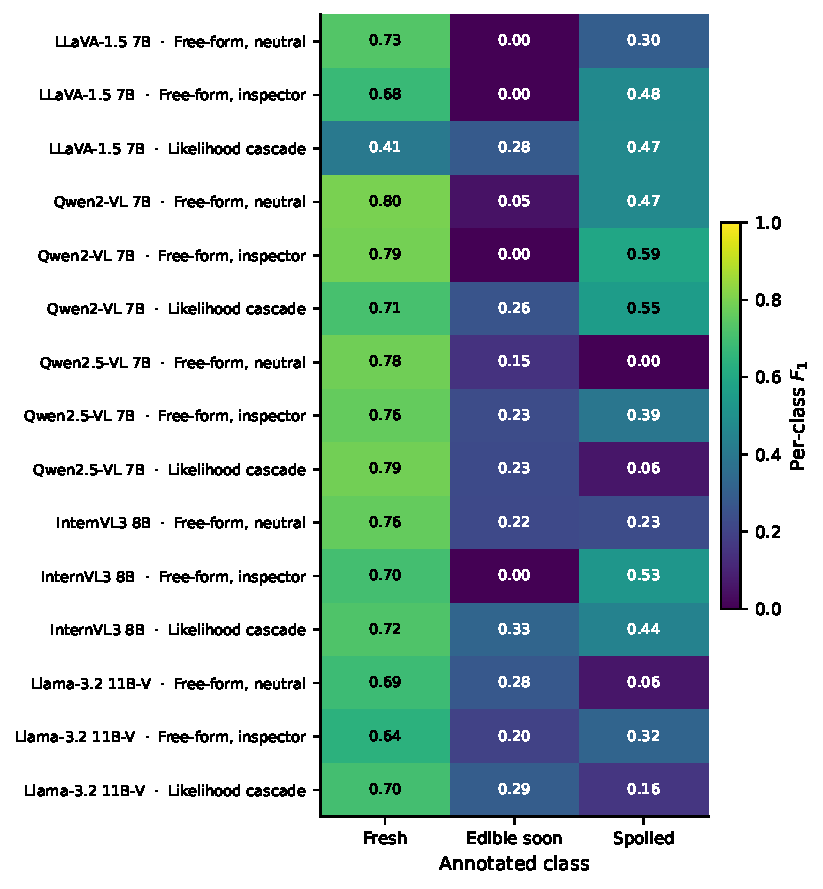
\includegraphics[width=0.72\textwidth]{figures/figure3.pdf}
\caption{Per-class $F_1$ for every model and querying strategy on the produce-condition task. The edible-soon column is the dominant failure: it never exceeds 0.33 and falls to exactly zero in four configurations, whereas fresh is recovered reliably throughout.}
\label{fig:perclass}
\end{figure}

% ---- figure4: confusion_pair ----
\begin{figure}[!htbp]
\centering
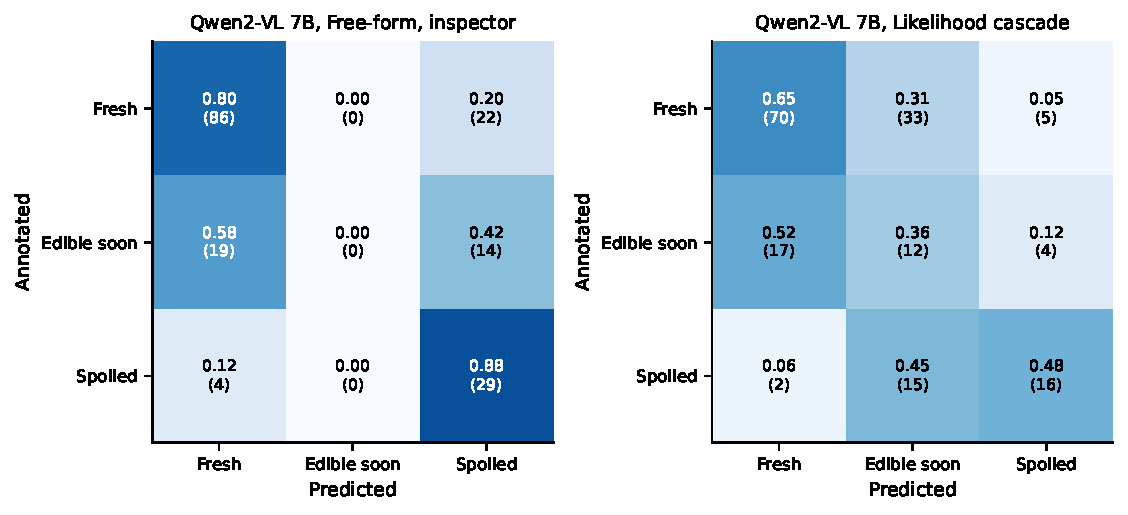
\includegraphics[width=\textwidth]{figures/figure4.pdf}
\caption{Row-normalised confusion matrices for Qwen2-VL 7B, the strongest model on this task, with raw counts in parentheses. Left: the rejection-oriented persona reaches high spoiled recall but assigns no item to edible soon, converting the three-class decision into a binary one. Right: the likelihood cascade recovers the intermediate class at the cost of overall accuracy.}
\label{fig:confusion}
\end{figure}

% ---- figure5: spoilage_roc ----
\begin{figure}[!htbp]
\centering
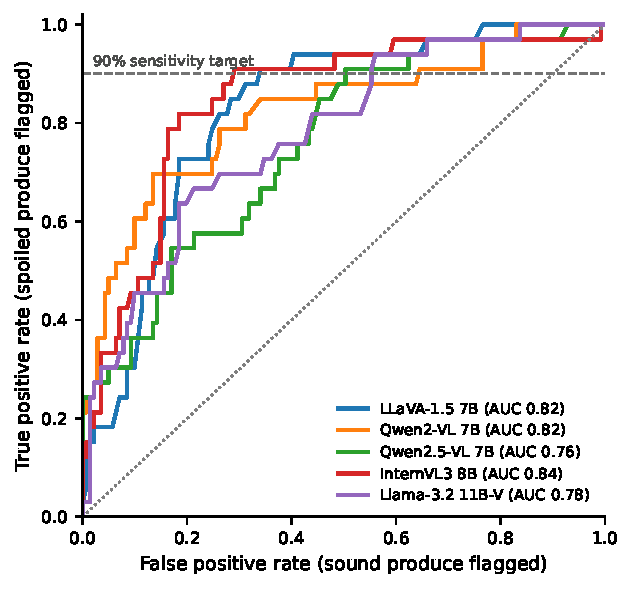
\includegraphics[width=0.58\textwidth]{figures/figure5.pdf}
\caption{Receiver operating characteristic curves for spoilage detection using the continuous cascade score $s_{\mathrm{spoil}}$ ($n = 174$, of which 33 are spoiled). All five models rank spoiled produce well above chance even though their fixed-threshold decisions are weak, which is what makes a ranked review queue viable where autonomous grading is not.}
\label{fig:roc}
\end{figure}

% ---- figure6: screening_tradeoff ----
\begin{figure}[!htbp]
\centering
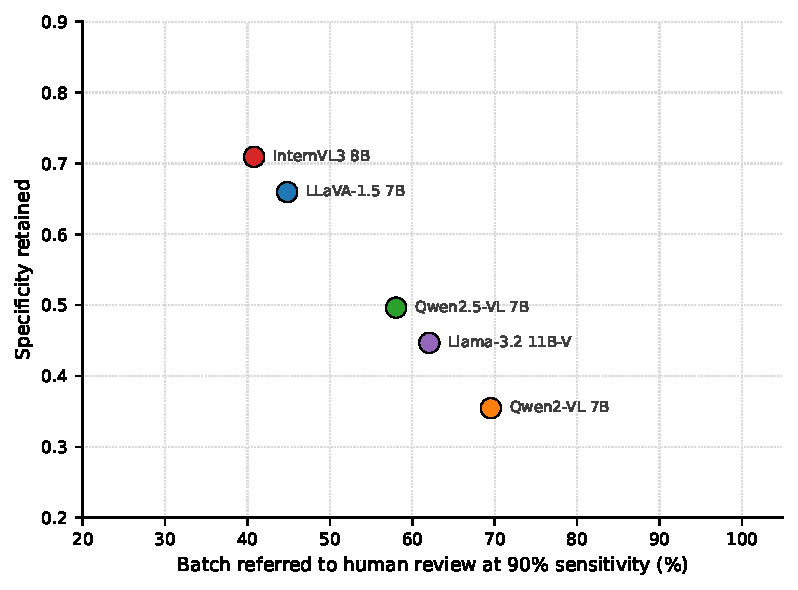
\includegraphics[width=0.6\textwidth]{figures/figure6.pdf}
\caption{Operating points with the cascade threshold set to achieve 90\% spoilage sensitivity. The horizontal axis is the share of the batch a human sorter must inspect and the vertical axis the specificity retained; upper-left is better. The model with the best macro-$F_1$ is not the best screen, which is why the deployment choice should be made on this plot rather than on a classification metric.}
\label{fig:screening}
\end{figure}

% ---- figure7: calibration ----
\begin{figure}[!htbp]
\centering
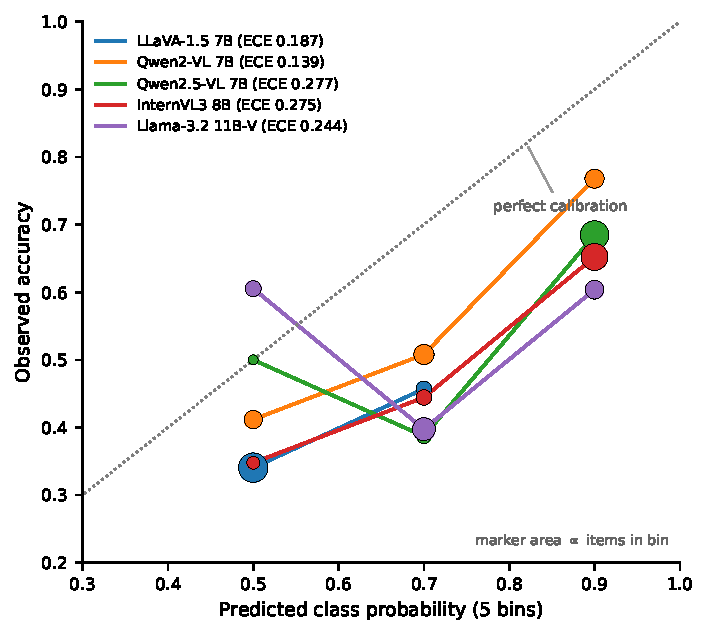
\includegraphics[width=0.58\textwidth]{figures/figure7.pdf}
\caption{Reliability diagram for the likelihood cascade, the only strategy that yields a per-item probability. Five display bins are used and marker area is proportional to the number of items in each bin; the quoted expected calibration error is computed at the standard ten bins. Points fall below the diagonal throughout, so the cascade is overconfident, but the ordering is monotone enough for the probability to serve as a deferral criterion.}
\label{fig:calibration}
\end{figure}

% ---- figure8: selective_prediction ----
\begin{figure}[!htbp]
\centering
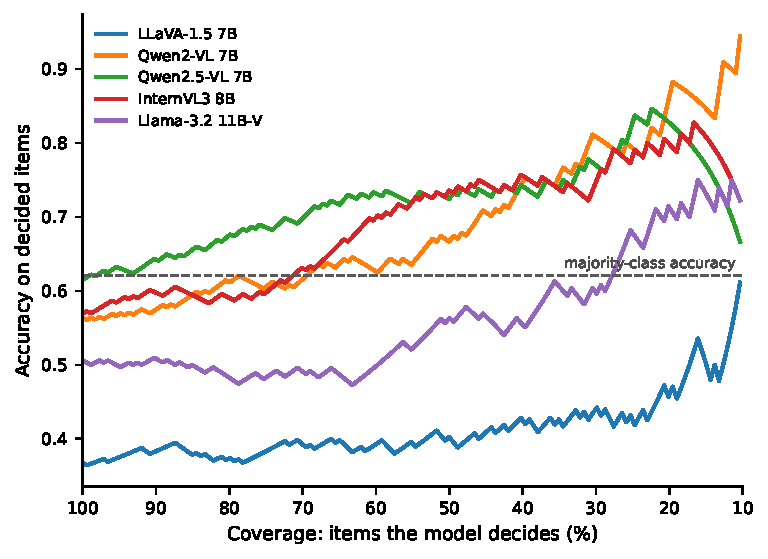
\includegraphics[width=0.62\textwidth]{figures/figure8.pdf}
\caption{Selective prediction with the likelihood cascade. Items are ranked by predicted class probability and the least confident are deferred to human review, so coverage decreases from right to left. Accuracy on the retained items rises as coverage falls, which is the behaviour a deferral policy depends on.}
\label{fig:selective}
\end{figure}

% ---- figure9: threshold_sweep ----
\begin{figure}[!htbp]
\centering
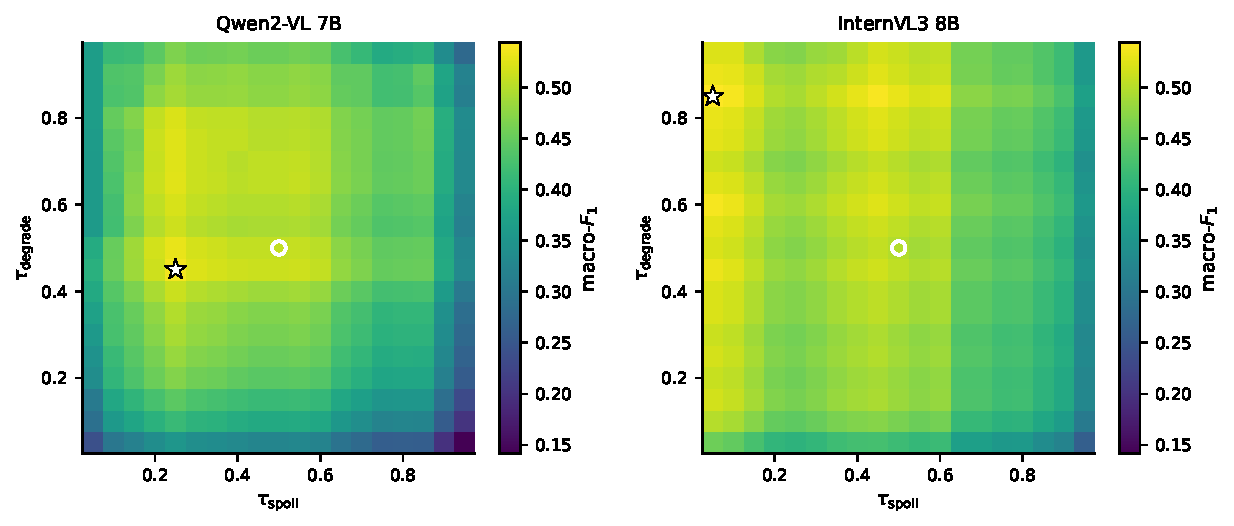
\includegraphics[width=\textwidth]{figures/figure9.pdf}
\caption{Macro-$F_1$ over the cascade threshold grid for the two strongest models. The open circle marks the default operating point $\tau = (0.5, 0.5)$ and the star the in-sample optimum. Performance varies more across thresholds within a single model than it does across models at a fixed threshold, so the threshold is a primary deployment parameter rather than an implementation detail.}
\label{fig:tau}
\end{figure}

% ---- figure10: defect_youden ----
\begin{figure}[!htbp]
\centering
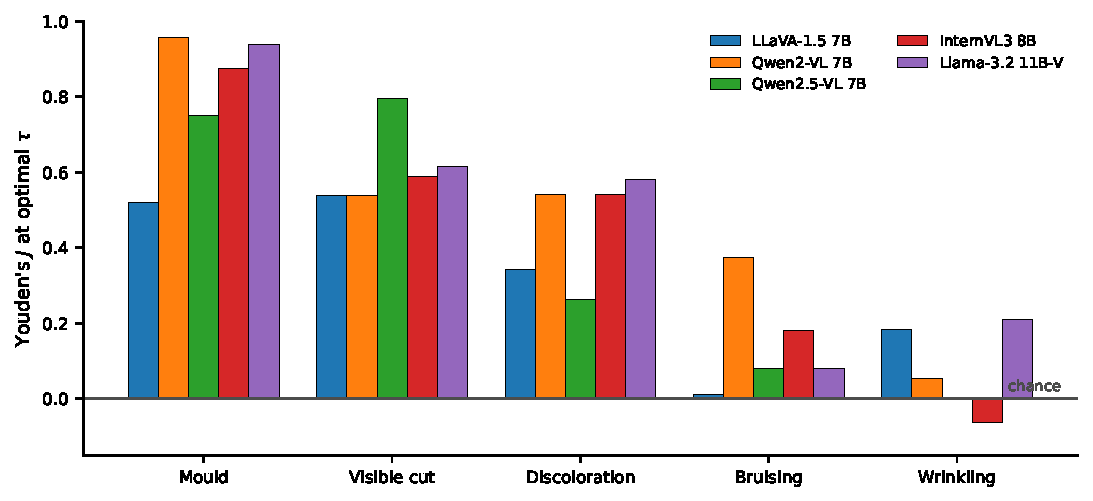
\includegraphics[width=\textwidth]{figures/figure10.pdf}
\caption{Youden's $J$ at the per-defect optimal threshold, by defect and model, on the defect-annotated produce subset. Values at or below zero indicate performance no better than chance. Mould is identified reliably while bruising and wrinkling are not. Thresholds are selected in sample, so these values are optimistic. Leaking is omitted because it has no positive instances in this subset.}
\label{fig:defects}
\end{figure}

% ---- figure11: accuracy_vs_latency ----
\begin{figure}[!htbp]
\centering
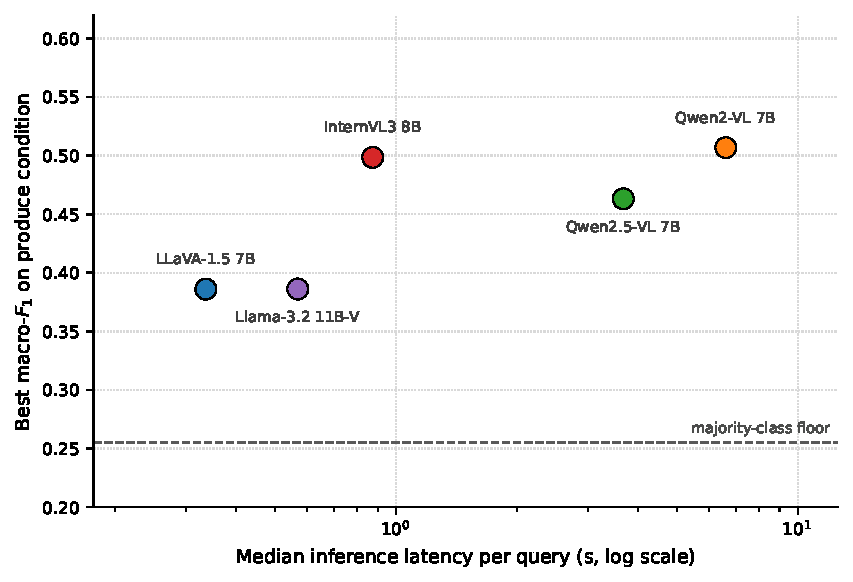
\includegraphics[width=0.6\textwidth]{figures/figure11.pdf}
\caption{Best produce-condition macro-$F_1$ against median inference latency on one NVIDIA A100 80GB GPU. Latency spans a twentyfold range while macro-$F_1$ spans roughly 0.12, so throughput rather than accuracy is likely to govern model choice at food-bank scale.}
\label{fig:latency}
\end{figure}
